\documentclass{article}
% Packages
\usepackage[utf8]{inputenc}
\usepackage{graphicx}
\usepackage{amsmath}
\usepackage{braket}
\usepackage[margin=0.7in]{geometry}
\usepackage[version=4]{mhchem}
% commands
\newcommand{\be}{\begin{equation}}
\newcommand{\ee}{\end{equation}}
\newcommand{\pd}{\partial}
% Title
\title{Chem132A: Final Solutions}
\author{Moises Romero, Shane Flynn}
\date{December 2017}
% End Set-up
\begin{document}

\maketitle

\section*{Question 1; 20 Points}

\subsection*{Arrhenius Equation}
For many biologically important reactions the rate of the reaction doubles if the temperature is increased by 10K from 298K to 308K. Calculate the activation energy for a reaction for which this is true.

\subsection*{Solution}
The Arrhenious Equaiton can be used to relate reaction rates and temperature. 
\be
k = Ae^{-\frac{E_a}{RT}}
\ee
We know the rate doubles, therefore we take a ratio and set it equal to two and solve. 
\be
\frac{k_2}{k_1} = 2 = \frac{A_2e^{-\frac{E_2}{RT_2}}}{A_1e^{-\frac{E_1}{RT_1}}}
\ee
If we assume the activation energy and Arrhenious constant are not a function of temperature we can simplify. 
\be
\ln(2) = \frac{-E_a}{R}\left(\frac{1}{T_2}-\frac{1}{T_1}\right)
\ee
Finally re-arrange and solve for the activation energy. 
\be
E_a = \frac{-R\ln(2)}{\left(\frac{1}{T_2}-\frac{1}{T_1}\right)} \approx 54\frac{kJ}{mol}
\ee

\subsection*{First Order Decay}
A radioactive isotope commonly used in biotracer studies of phosphorous metabolism is $^{32}$P, which has a decay half-life of 14.3 days.
Suppose we have been doing experiments with $^{32}$P and accumulate waste material that is showing a radioactive decay rate of 3.7 x 10$^7$ decays per second.
The radiation safety officer of the University rules that it is not safe to dispose of this waste material until the decay rate has decreased to 3.7 x 10$^2$ decays per second. 
Until the rate has decreased sufficiently, it must be stored in a lead container in our laboratory. 
How many days must we store the waste in the lead container before it is safe to dispose of it?

\subsection*{Solution}
To solve this problem we need to realize that any type of radioactive decay is a First-Order decay process.
We can therefore solve for the half-life of the decay and find the rate. 
\be
\begin{split}
    \frac{d}{dt}[x] &= -k[x]\\
    \int_{x_0}^{x_0/2} \frac{d[x]}{[x]} &= \int_0^t-kdt\\
    \ln\left(\frac{x_0/2}{x_0}\right) &= -kt\\
    k = \frac{\ln(2)}{t} &= \frac{\ln(2)}{14.3} \approx 0.0485 \text{day}^{-1}
\end{split}
\ee
Now that we have the rate (assuming it will be constant throughout the decay) we can solve for the time of a generic first order decay (not the half-life time now). 
\be
\begin{split}
    -kt &= \ln\left(\frac{[^{32}P]}{[^{32}P]_0}\right) \\
    t &= -\frac{1}{k}\ln\left(\frac{[^{32}P]}{[^{32}P]_0}\right)\\
        t &= -\frac{1}{0.0485}\ln\left(\frac{3.7 \times 10^2}{3.7\times 10^7}\right) \approx 237\text{days}
\end{split}
\ee


\newpage

\section*{Question 2; 30 Points}
The overall reaction $\ce{O2NNH2}$(aq) $\ce{<=>}$ N$_2$O(aq) + H$_2$O(l) occurs in water solution by the set of elementary steps shown below. Determine the rate law that is consistent with this mechanism.

\be
\begin{split}
    \ce{O2NNH2 <=>[\ce{k_1}][\ce{k_{-1}}] O2NNH^- + H^+} &\qquad \qquad \text{fast equilibrium}\\
    \ce{O2NNH^- ->[\ce{k_2}]} N2O + OH^- &\qquad \qquad \text{slow}\\
    \ce{H^+ + OH^- ->[\ce{k_3}] H2O} &\qquad \qquad \text{fast}
\end{split}
\ee

\subsection*{Solution}
We assume that the overall rate of the reaction is dictated by the slowest step in the provided mechanism. 
Because the slow step of the mechanism only has a reaction arrow in one direction we write the rate in terms of the reactants. 
\be
Rate = k_2[O_2NNH^-]
\ee
This rate is in terms of a reaction intermediate which is not proper form, so we make a steady state approximation on this intermediate.
For the exam it was sufficient to simply use the fast equilibrium to substitute in. 
\be
Rate_1 = k_1[O_2NNH_2] = k_{-1}[O_2NNH^-][H^+] \Rightarrow [O_2NNH^-] = \frac{k_1}{k_{-1}[H^+]}[O_2NNH_2]
\ee
Therefore we can write the rate in terms of 
\be
Rate = \frac{k_1k_2}{k_{-1}}\frac{[O_2NNH_2]}{[H^+]}
\ee

\newpage

\section*{Question 3; 30 Points}
The table below shows the results from four experiments that were done to discover how the initial rate of consumption of BrO$_3^–$(aq) ions varies as the concentrations of the reactants are changed in the following reaction:
\be
\ce{BrO3^- + 5Br^- + 6H3O^+ <=> 3Br2 + 9H2O}
\ee

The following data at 300K is available (all in terms of initial concentration):

\begin{center}
  \begin{tabular}{ | l | c | r | q | h | }
    \hline
    Exp. & [BrO$_3^-$] & [Br$^-$] & [H$_3$O$^+$] & Initial Rate \\ \hline
    1 & 0.10 & 0.10 & 0.10 & 1.2 $\times$ 10$^{-3}$ \\ \hline
   2 & 0.20 & 0.10 & 0.10 & 2.4 $\times$ 10$^{-3}$ \\ \hline
    3 & 0.10 & 0.30 & 0.10 & 3.5 $\times$ 10$^{-3}$ \\ \hline
    4 & 0.20 & 0.10 & 0.15 & 5.5 $\times$ 10$^{-3}$ \\ \hline
  \end{tabular}
\end{center}

\subsection*{Reaction Order}
Determine the order of the reaction with respect to each reactant. 
Indicate which pair of experiments you used to arrive at each of your answers. 

\subsection*{Solution}
We could do this a bit more formally, but we can determine the reaction order by simple observation for these numbers. 
In general we expect
\be
Rate = k[BrO_3^-]^x[Br^-]^y[H_3O^+]^z
\ee
Comparing Experiment 1 with Experiment 2 we see doubling the concentration of $BrO_3^-$ causes the rate to double, therefore the reaction is First-Order wrt $BrO_3^-$. 
Again comparing Experiment 1 with Experiment 3 we see that tripling the concentration of Br$^-$ causes the rate to triple, again making the overall reaction First Order wrt Br$^-$. 
Finally, comparing Experiment 2 with Experiment 4 we see that half an increment increases causes the rate to double, therefore the reaction is Second Order wrt H$_3$O$^+$.  
\be
Rate = k[BrO_3^-][Br^-][H_3O^+]^2
\ee

\subsection*{Rate Law}
Write the rate law for the reaction in terms of $\frac{d}{dt}$[Br$_2$].
Calculate the rate constant at 300K (Indicate what data you use from the table for determining k). 

\subsection*{Solution}
Using the stoichometry of the reaction (and Part 1) we can write the following rate law. 
\be
Rate = \frac{1}{3}\frac{d}{dt}[Br_2] = k[BrO_3^-][Br^-][H_3O^+]^2
\ee
Using the first experiment we can easily solve for the value of k. 
\be
\begin{split}
1.2 \times 10^{-3} &= 3k (0.1)(0.1)(0.1)^2 \\
k &= \frac{1.2 \times 10^{-3}}{3(0.1)^4} \approx 4M^{-3}s^{-1}
\end{split}
\ee

\newpage

\section*{Question 4; 30 Points}

\subsection*{Ideal Gas}
1 mole of an ideal gas is heated from T$_1$ to T$_2$ in a rigid container (constant volume).
This process is done reversibly.
Calculate the heat (q), work (w), change in Internal Energy ($\Delta$U), and the change in Entropy ($\Delta$S) associated with the process. 

\subsection*{Solution}
Since this is an isochoric process there is no change in volume. 
\be
\Delta V = 0 
\ee
Without a volume change, the work must be 0. 
\be
w=0
\ee
For an ideal gas, the Internal Energy is only a function of temperature.
Therefore we can re-write the First Law as : 
\be
\Delta U = q = \int_{T_1}^{T_2}C_vdT
\ee
Finally our expression for the Entropy of a reversible process is: 
\be
\Delta S = \frac{q_{rev}}{T} = \int_{T_1}^{T_2}\frac{C_vdT}{T}
\ee

\subsection*{Nonideal Gas}
1 mol of a gas described by the Virial equation of state, undergoes a reversible isothermal expansion.
\be
P=\frac{RT}{V_m}\left(1 + \frac{B}{V_m}\right)
\ee
For this system Internal Energy is only a function of temperature.
Calculate the heat (q), work (w), change in Internal Energy ($\Delta$U), and change in Entropy ($\Delta$S).  

\subsection*{Solution}
We are told this is an isothermal process therefore: 
\be
\Delta T = 0
\ee
Because the Internal Energy is only a function of Temperature we also know that
\be
\Delta U = 0 
\ee
Knowing this the first law can be expressed as : 
\be
q=-w
\ee
The process is reversible meaning  P$_{ext}$ = P$_{gas}$.
\be
q=-w=\int_{V_1}^{V_2} P_{ext} =  \int_{V_1}^{V_2} P_{gas}=\int_{V_1}^{V_2} \frac{RT}{V_m}\left(1 + \frac{B}{V_m}\right)
\ee
Since we have 1 mol of gas V$_m$ = V. 
\be
q=-w=\int_{V_1}^{V_2} \left(\frac{RT}{V}+ \frac{RTB}{V^2}\right) = \int_{V_1}^{V_2} \frac{RT}{V} +  \int_{V_1}^{V_2} \frac{RTB}{V^2} =  RT\int_{V_1}^{V_2} \frac{1}{V} +  RTB\int_{V_1}^{V_2} \frac{1}{V^2} 
\ee
Finally we see that 
\be
q=-w= RT\ln\frac{V_2}{V_1} + RTB\left(-\frac{1}{V_2} + \frac{1}{V_1}\right)
\ee

The process is done reversibly therefore
\be
\Delta S = \frac{q_{rev}}{T} = \frac{RT\ln\frac{V_2}{V_1} + RTB\left(-\frac{1}{V_2} + \frac{1}{V_1}\right)}{T} = Rln\frac{V_2}{V_1} + RB\left(-\frac{1}{V_2} + \frac{1}{V_1}\right)
\ee

\subsection*{Adiabatic Process}
A gas undergoes an adiabatic compression in which the volume drops to $\frac{1}{2}$ its original value. 
The pressure of the gas increases by a factor of 4. What is the specific heat ratio?

\subsection*{Solution}
For an adiabatic process (ideal gas) we can use the following expression : 
\be
P_1V_1^\gamma=P_2V_2^\gamma
\ee
Where $\gamma$ is the specific heat ratio.
From the problem we can express the ratio of P$_1$ to P$_2$ as : 
\be
\frac{P_2}{P_1} = 4 
\ee
We can then express the initial volume to final volume as:
\be
\frac{V_2}{V_1} = \frac{1}{2} 
\ee
However when we rearrange the equation we will need the inverse of this so : 
\be
\frac{V_1}{V_2} = 2 
\ee
We can then rearrange the initial equation as : 
\be
\frac{P_2}{P_1} = \left(\frac{V_1}{V_2}\right)^\gamma
\ee
We can plug in our values to simplify : 
\be
4=2^\gamma
\ee
We can now take the logarithm of each side and rearrange to solve for $\gamma$: 
\be
\gamma = \frac{\ln4}{\ln2} = 2 
\ee

\subsection*{Free Expansion}
A gas expands into a vacuum from an initial volume to a final volume. 
Upon reaching the final volume there is no measured change in temperature. 
\bigskip

Does Entropy increase , decrease, or stay the same? Justify your answer.
What is the work for this process? Justify your answer. 
Is this a reversible or irreversible process? Justify your answer.

\subsection*{Solution}
Entropy increases as the gas particles are expanding into a larger volume which generates more microstates available to the system.

\subsection*{Solution}
By definition of a free expansion the work is zero, there is no external pressure applied by the vacuum. 

\subsection*{Solution}
This is an irreversible process as the gas goes through states of non-thermodynamic equilibrium (the movie cannot be played in reverse). 

\newpage

\section*{Question 5; 30 Points}

Consider the combustion of benzene gas under constant pressure conditions (1atm) and at temperature of 400K. The balanced reaction for this combustion is given. Using the data provided calculate the $\Delta H_{rxn}$(370K). 

\be
2C_6H_6(gas) + 15O_2(gas) \longrightarrow 12CO_2(gas) + 6H_2O (liquid)
\ee

For benzene (\textbf{liquid}) the following data is available:
\bigskip

$\Delta H^o_{f}$(298) = 49kJmol$^{-1}$
\bigskip

$\Delta H^o_{vap}$ = 33.9kJmol$^{-1}$
\bigskip

Boiling Point = 353.2K
\bigskip

Cp(benzene liquid) = 136.1Jmol$^{-1}$K$^{-1}$
\bigskip

Cp(benzene gas) = 81.67Jmol$^{-1}$K$^{-1}$
\bigskip

For O$_2$(gas) : \\
$\Delta H^o_{f}$(298) = 0\\ 
Cp = 29.355Jmol$^{-1}$K$^{-1}$
\bigskip

For CO$_2$(gas) :\\
$\Delta H^o_{f}$(298) = -393.51kJmol$^{-1}$\\
Cp =37.11Jmol$^{-1}$K$^{-1}$
\bigskip

For H$_2$O(liquid) :\\
$\Delta H^o_{f}$(298) = -285.83kJmol$^{-1}$\\
Cp = 75.291Jmol$^{-1}$K$^{-1}$
\bigskip

Show your reasoning and all work for full credit.

\subsection*{Solution}
\subsection*{Formation of Benzene Gas}
We are only given information about the liquid state of benzene, we need the enthalpy of formation for benzene gas. 
This is found by taking the formation enthalpy of the liquid, heating the liquid to the normal boiling point, doing the phase transition to a  gas, and then heating the gas to the final temperature. 
\be
\begin{split}
\Delta H(\text{Benzene},370,g) &= \Delta H_f(298,l) + \Delta H(l,298\Rightarrow 353.2) + \Delta H_{vap}(353.2) + \Delta H(g, 353.2 \Rightarrow 370)\\
&= 49 + \int_{298}^{353.2} C_P(l)dT + 33.9 + \int_{353.2}^{370} C_P(g) dT \\ 
&= 49 + 0.1361(353.2-298) + 33.9 + 0.08167(370-353.2) \\
\Delta H(\text{Benzene},370,g) &= 91.78 \frac{\text{kJ}}{\text{mol}}
\end{split}
\ee

\subsection*{Oxygen Gas}


\be
\begin{split}
\Delta H(O_2,g, 370) &= \Delta H_f(298,g) + \int_{298}^{370} C_P(g)dT\\
&= 0 + 0.029355(370-298)\\
\Delta H(O_2,g, 370) &= 2.11356
\end{split}
\ee

\subsection*{Carbon Dioxide Gas}

\be
\begin{split}
\Delta H(CO_2,g, 370) &= \Delta H_f(298,g) + \int_{298}^{370} C_P(g)dT\\
&= -393.51 + 0.03711(370-298)\\
\Delta H(CO_2,g, 370) &= -390.83808
\end{split}
\ee

\subsection*{Water Liquid}
\be
\begin{split}
\Delta H(H_2O,l, 370) &= \Delta H_f(298,l) + \int_{298}^{370} C_P(l)dT\\
&= -285.83 + 0.075291(370-298)\\
\Delta H(H_2O,g, 370) &= -280.4090
\end{split}
\ee

\subsection*{Reaction}
Now that we have calculated the Enthalpy associated with each component at the final temperature, we simple need to subtract values. 

\be
\begin{split}
\Delta H_{\text{rxn}}(370) &= \sum_i \nu_i \Delta H_i \\
&= 12(\Delta H(CO_2,g, 370)) + 6(\Delta H(H_2O,l, 370)) - 15(\Delta H(O_2,g, 370)) - 2(\Delta H(\text{Benzene},370,g)) \\
&= 12(-390.8380) + 6(-280.4090) - 15(2.1135) - 2(91.78) \\
\Delta H_{\text{rxn}}(400) &= -6587.7725 \frac{\text{kJ}}{\text{mol}}
\end{split}
\ee

\newpage

\section*{Question 6; 30 Points}
\subsection*{Single Component Phase Diagram}
In this question we will characterize the phase diagram of a single component system. 
This phase diagram contains two different solid phases ($\alpha$, and $\beta$).
The $\alpha$ phase is more stable at lower temperatures. 

Label the phase diagram (write on the graph) to the best of your ability. 
Be sure to Label all of the physical phases in the system.
Label the transitions occurring at each phase line.
And for each phase, phase line, and triple point, make a statement about the associated chemical potentials. 

\subsection*{Solution}
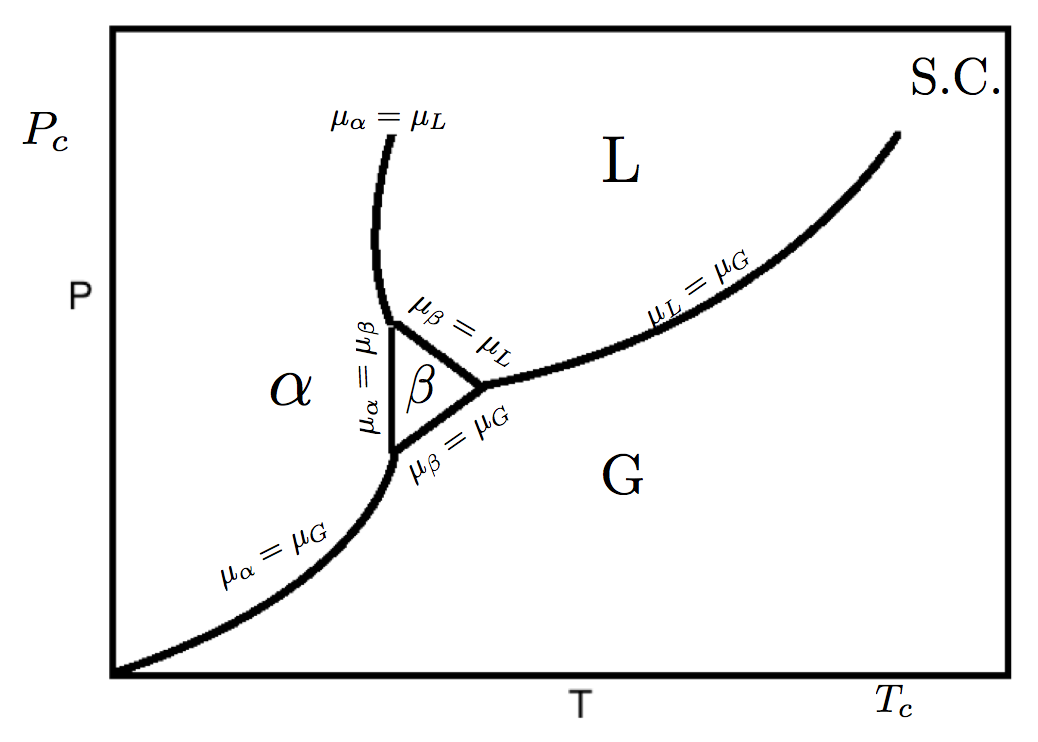
\includegraphics{ps6_soln.png}

For each individual phase, that phase has the lowest chemical potential at the given pressure and temperature. 
There are also 3 triple points on the graph (the three vertices of the triangle). 
At each triple point the three phases must all have the same chemical potential and it must be lower than every other Chemical Potential in the system. 
For transitions you simply needed to state which transition was occurring; $\alpha$ to $\beta$, L to G and etc (formal names were accepted but not necessary). 

\newpage 

\subsection*{First Order Phase Transition}
In the graphs below sketch the indicated molar quantities as a function of temperature (T$_b$ is the boiling temperature). 

\subsection*{Solution}
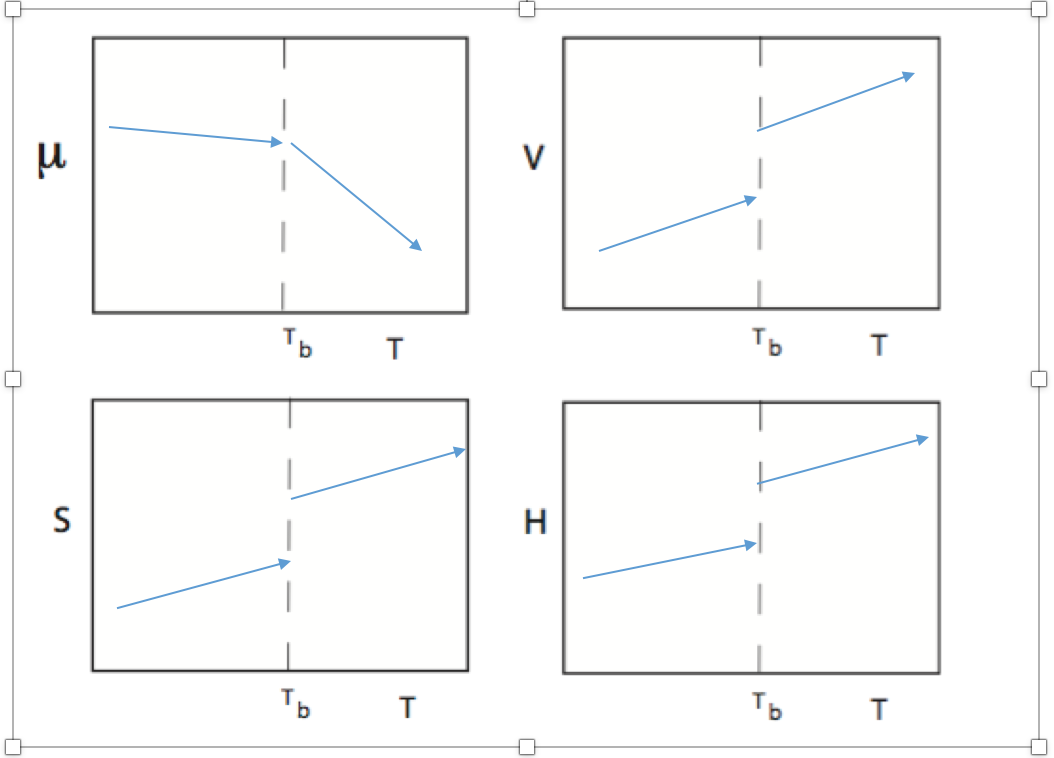
\includegraphics{b_ps6.png}

We are going through a phase transition (liquid to gas, assume constant pressure). 
We know that the chemical potential is minimized, it therefore must decrease upon transition. 
Intuitively the volume of a gas is larger than a liquid (it fills its container), therefore we see a discontinuity at the transition.
The others can all be derived in a similar manner. 

\newpage

\section*{Question 7; Flux}

\subsection*{Dimensions}
In general, what are the physical dimensions of flux?

Please draw a simple picture to help illustrate your answer. 

\subsection*{Solution}
In general the flux (basic definition 3D) is simply the amount  of some substance ($\equiv$ X) traveling through a given (constant) area during some time interval. 
\be
\text{Flux} = \frac{X}{A \enskip t}
\ee
The picture should just be some shape with an arrow showing 'stuff' going through it (perpendicular to the geometry). 

\subsection*{Flux in Thermodynamics}
During lecture we discussed various transport properties of interest to chemical systems. 
The various types of flux (J) are usually proportional to a spatial derivative.
\be
J(\text{Some Property}) = c\frac{d}{dz}f(x,y,z)
\ee
Where the coefficient c relates the proportionality. 
These coefficients are well-known and can be tabulated for various materials. 
The function f is the variable that is actually changing during the flux.

Given the three following transport coefficients, please write down the analogous Fick's Law equation.

To do this you will need to define the type of flux that is associated with the transport coefficient, and the physical variable that is changing during that flux. 
Be sure to define all symbols used, and briefly explain each type of flux in words.  

\begin{enumerate}
\item The Diffusion Coefficient (D)
\item The Thermal Conductivity Coefficient ($\kappa$)
\item The Viscosity Coefficient ($\eta$).
\end{enumerate}

\subsection*{Solution}
For this question we are asked to construct an equation similar to Fick's Law for each coefficient.
We need to define what property of flux we are measuring with that coefficient. 

The diffusion coefficient is associated with the flux of matter in our system.
I will use the generic variable J to define flux.
\be
J(\text{matter}) = -D \frac{d}{dz} \mathcal{N}
\ee
Where $\mathcal{N}$ is the number density of the molecules. 
Because concentration travels down its  gradient (i.e. higher concentration to lower) we need a minus sign. 
And the matter flux measures how things (atoms/molecules) propagate throughout the system. 

The thermal conductivity coefficient is  related  to the flux of thermal energy (thermal motion). 
\be
J(\text{Thermal Motion}) = -\kappa \frac{d}{dz} T
\ee
And it measures how the temperature propagates throughout the system. 

Finally we have the Viscosity Coefficient which is related to the flux in linear momentum. 
\be
J(\text{Linear Momentum}) = -\eta \frac{d}{dz} m\nu_x
\ee
The flux of linear momentum measures the momentum distribution of particles throughout the system. 

\subsection*{Collision Flux}
For a perfect gas the collision flux (Z$_w$) can be shown to be 
\be
Z_w = \frac{P}{\sqrt{2\pi mk_BT}}
\ee
Where P is the pressure of the gas, m is the mass, k$_B$ is Boltzmann's constant, and T is the temperature of the gas. 

Using dimensional analysis show that this equation is reasonable (i.e. show the units of each side of the equation are consistent). 

\vspace{10pt}

\textbf{Note:} The units of k$_B$ are $\frac{m^2 kg}{s^2 K}$, and a Newton (the unit of force) is $\frac{kg \enskip m}{s^2}$.

\subsection*{Solution}
The collision flux measures how often the molecules strike a region in the gas. 
We can write the LHS of the equation as an amount (X) per area-time.
Pressure (P) is intuitively defined as Force/Area.
\be
\begin{split}
Z_w &= \frac{P}{\sqrt{2\pi mkT}}\\
\frac{X}{A t} &= \frac{\frac{N}{A}}{\sqrt{mkT}}\\
\frac{X}{A t} &= \frac{\frac{kg \enskip m}{s^2m^2}}{\sqrt{kg \frac{m^2\enskip kg}{s^2\enskip K}K}}\\
\frac{X}{m^2 s} &= \frac{\frac{kg}{s^2m}}{\frac{kg \enskip m}{s}}\\
\frac{X}{m^2 s} &= \frac{1}{m^2s}
\end{split}
\ee
From our analysis this definition does seem reasonable, we learn that the quantity X (our flux) does not actually carry any units, but is consistent with the dimensions of flux. 


\subsection*{Collisions}
Consider a rectangular surface exposed to an argon gas. 
Determine the number of collisions that occur with the surface over the time interval t. 

\subsection*{Solution}
If the collision flux determines the number of collisions that occur in an area-time, then the number of collisions (X) with some area-time interval must be
\be
X = Z_w A t
\ee
We know that area of the collisions is a rectangle therefore A = l*w. 
We can also write down the mass of argon in terms of the molar mass and Avogadro's number, $m=\frac{M}{N_A}$.
Making these substitutions we find
\be
X = \frac{Plwt}{\sqrt{\frac{2\pi Mk_BT}{N_A} }}
\ee

Please note: many (most) students tried to use the equations developed for collisions occurring in ideal gases according to the Maxwell Boltzmann Distribution. 
This is not relevant to the question being asked, it is simply trying to run to equations!

\end{document}